%!TEX root = document.tex

%%%%%%%%%%%%%%%%%%%%%%%%%%%%%%%%%%%%%%%%%%%%%%%%%%%%%%%%%%%%%%
\begin{figure}[t!]
\centering
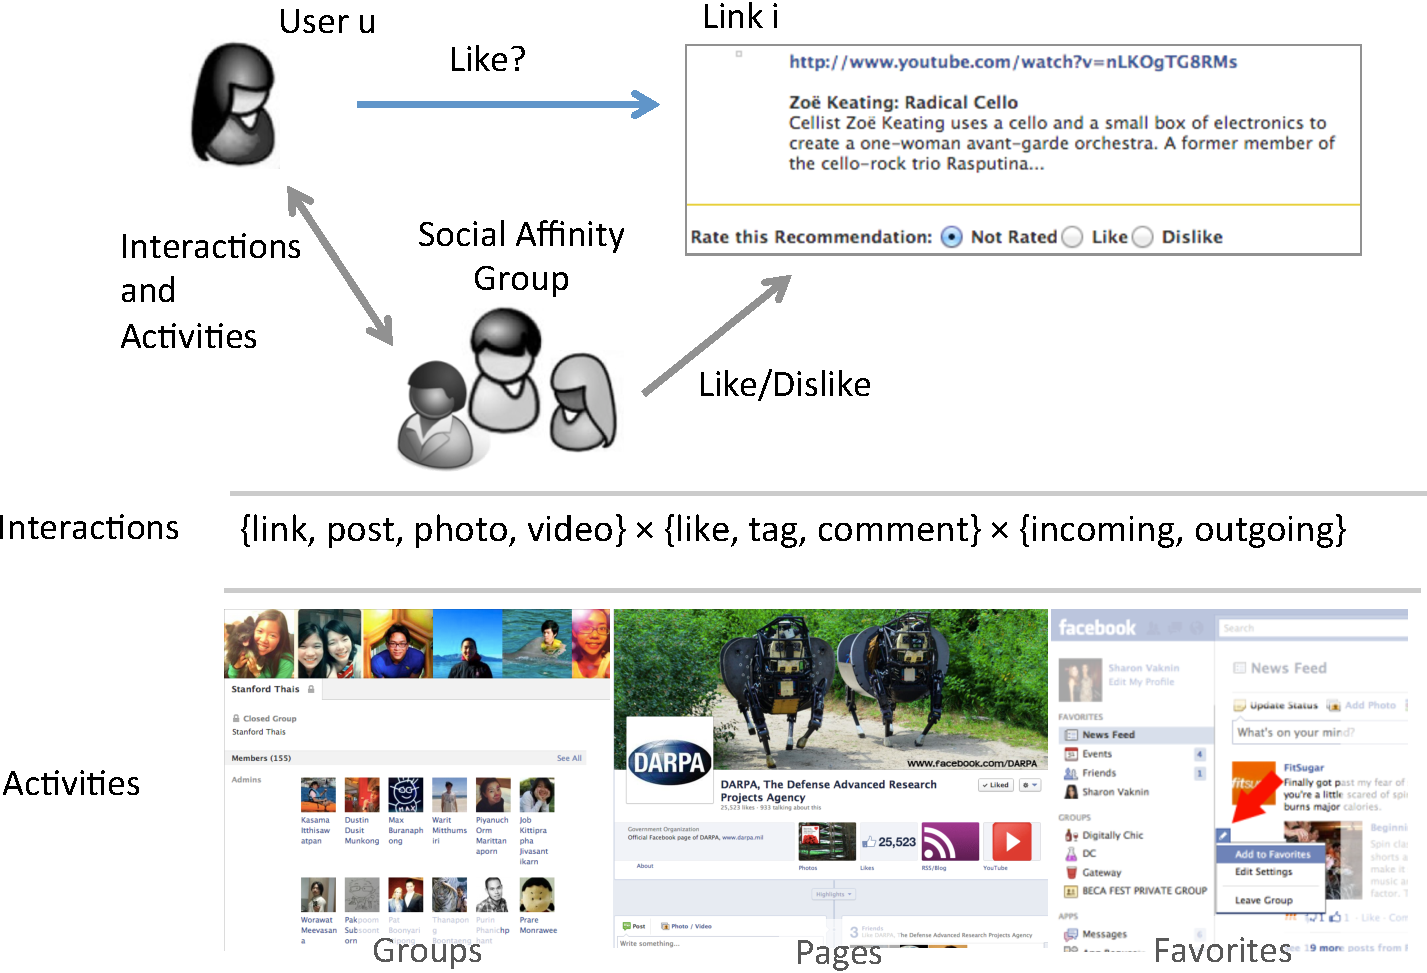
\includegraphics[width=1\linewidth]{data/overview}
\caption{Overview of \emph{social affinity filtering (SAF)}: A
  \emph{social affinity group (SAG)} of user $u$ (ego) consists of a
  set of alternate users $\{ v \}$ (alters) who have a certain
  \emph{interaction} or share an \emph{activity} membership with $u$.
  SAF learns to classify whether user $u$ will like item $i$ based on
  the observed preferences of members of each SAG of user $u$
  toward item $i$.}
\label{fig:overview}
\end{figure}
%%%%%%%%%%%%%%%%%%%%%%%%%%%%%%%%%%%%%%%%%%%%%%%%%%%%%%%%%%%%%%

As illustrated in Fig~\ref{fig:overview}, the high-level objective of
this work is to predict whether or not a user $u$ (ego) will like an item
$i$.  Specifically, the Facebook App
we have built for our experimentation collects explicit like and
dislike feedback for links posted on Facebook
(e.g., Youtube video, news or blog item, etc.) leading to the following
preference data:
\begin{align*}
\like(u,i) & \! := \! 
          \begin{cases}
	  \true    \!\! & \!\! \text{$u$ clicked \emph{like} for $i$}\\
	  \false   \!\! & \!\! \text{$u$ clicked \emph{dislike} for $i$}\\
          \unknown \!\! & \!\! \text{$u$'s preference for $i$ is unobserved}
	  \end{cases}
\end{align*}
From the observed data, \emph{social affinity filtering (SAF)}
learns to predict $\like(u,i)$ based on the surrogate link
preferences $\like(v,i)$ of sets of other Facebook users $v$ who have
at least one interaction or activity in common with $u$.  The details
of SAF are outlined in the following subsections.
%On Facebook,
%there are many possible fine-grained interactions and activities
%as outlined next.

\subsection{Interactions and Activities on Facebook}

In the context of Facebook, we use the term {\em interactions} and
{\em activities} to refer to the range of user-user and user-community
actions, respectively.

\vspace{3mm}

\noindent {\bf Interactions} describes communication between Facebook users
and can be broken down into the following dimensions:

\begin{itemize}

\item \textbf{Modality:} (4 possibilities) User $u$ can interact with
  another user $v$ via \textit{links, posts, photos} and
  \textit{videos} that appear in either user's timeline.

\item \textbf{Action type:} (3 possibilities) A user $u$ can
  \textit{comment} or \textit{like} user $v$'s item. He/she can also
  \textit{tag} user $v$ on an item, often indicating that user $v$ is
  present when the content is created (for photo/video/post), or to
  explicitly raise user $v$'s attention for a post --- with one
  exception in Facebook that $u$ cannot tag a link with users.

\item \textbf{Directionality:} (2 possibilities) We look at
  \textit{incoming} and \textit{outgoing} interactions, i.e., if user
  $u$ comments on, tags, or likes user $v$'s item, then this is an
  \textit{outgoing} interaction for $u$, and an \textit{incoming} 
  interaction for $v$.
  Although high correlation between \textit{incoming} and
  \textit{outgoing} interactions has been
  observed~\cite{saez2011high}, whether interaction direction affects
  user preferences differently is still an open question we wish to
  answer in this work.

\end{itemize}

Overall there are 22 possible interaction types, namely the cross-product of modalities, actions and directions, minus the special cases of {\em link-tag-\{incoming, outgoing\}} since links cannot be tagged.

\vspace{3mm}

\noindent {\bf Activities} are user interactions with Facebook
communities like groups, pages, and favourites defined as follows:
\begin{itemize}
  \item \textbf{Groups} on Facebook 
\footnote{From Facebook Blog: 
\surl{http://www.facebook.com/blog/blog.php?post=324706977130}, ``Groups are the place for small group communication and for people to share their common interests and express their opinion. Groups allow people to come together around a common cause, issue or activity to organise, express objectives, discuss issues, post photos and share related content.'' 
\label{fn:fbblog}}
are analogous to real-world community organisations.  They allow 
  users to declare membership and support people to organise
  activities, to post related content, and to have recurring
  discussions about them.  Examples of groups include {\em Stanford
  Thai} (Fig~\ref{fig:overview} bottom left), or {\em Harvard Debate
  Club}.  

\item \textbf{Pages} on Facebook \footnote{From Facebook
  Blog:
  (\surl{http://www.facebook.com/blog/blog.php?post=324706977130}
  ``Facebook Pages enable public figures, businesses, organisations
  and other entities to create an authentic and public presence on
  Facebook. Facebook Pages are visible to everyone on the Internet by
  default. Facebook users can connect with these Pages by becoming a
  fan and then receive their updates and interact with them.'' }
  %\footnotemark[\ref{fn:fbblog}] 
  are analogous to the homepages of people, organisations and events
  on the world-wide-web. They are publicly visible, and users can
  subscribe to the updates on the page, and also engage in
  discussions. Example pages include {\em DARPA} (an organisation,
  Fig~\ref{fig:overview} bottom middle), or {\em Beyonce} (a singer).

  \item \textbf{Favourites} are analogous to bookmarks (on physical
  books or on the web browser).  They are a user-created list containing
  various items such as Facebook apps, books, music, and many other
  types of items (even pages) to indicate their interest.  Example favourites 
  include {\em Big Bang Theory} (TV series), or {\em FC Barcelona}
  (soccer club). Fig~\ref{fig:overview} bottom right shows a Facebook
  screenshot when a user adds a favourite.  \footnote{According to
  Facebook Blog, (\surl{https://www.facebook.com/help/232262810142682}
  ``Facebook facilitates a wide variety of user selected favourites
  (Activities, Favorite Athletes, Books, Interests, Movies, Music,
  Sports, Favorite Teams, Television). These favourites allow a user
  to associate themselves with other people who share their same
  favourite tendencies.''}
\end{itemize} 

Our evaluation includes 3000+ {\em group}, 4000+ {\em page} and
10000+ {\em favourite} features as detailed in
Sec~\ref{sec:datadesc}.

%% Good, but probably better in related work.  -SPS
\eat{
Note that the notion of affinity we adopt is based on direct user {\em
actions}, rather than static profile information, or structural
information of the social graph.  We believe this is a useful view
into the social network, as it was recently pointed out that a user's
attention (i.e., interactions) are divided among a small subset of
Facebook friends~\cite{backstrom2011center}, and that ratings of
real-world friendship strength seems to be more predictable from the
intimacy, intensity, and duration of interactions, than from social
distance and structural information~\cite{gilbert2009predicting}. Our
affinity definition is based on direct interactions within a users'
ego network, this is complementary to a recent
alternative~\cite{Panigrahy2012ubr} that uses number of paths between
two users to encode the resilience of network structure, as it was
recently found~\cite{Goel2012structure} that the vast majority of
information diffusion happens within one step from the source node. }
%Our affinity \cite{Wilson2012BSG}

\subsection{Social Affinity Groups (SAGs)}
\label{ssec:sag}

With {\em interactions} and {\em activities} now defined, we proceed to 
define two types of {\em social affinity groups (SAGs)} of a user $u$
that will be used as proxies for $u$'s preferences:

\begin{itemize}
  \item \textbf{Interaction Social Affinity Groups (ISAGs)}: Let the set of
  ISAGs be the cross-product of interaction
  modality, action, and direction:
  \begin{align*}
  	\textit{Interaction-Classes} := \, & \{\link, \post, \photo, \video\} \\
                                           & \times \{\like, \ttag, \comment\} \\
                                           & \times \{\incoming, \outgoing\}
  \end{align*}
  Then for $k \in \textit{Interaction-Classes}$ we define 
  \begin{align*}
     \textit{ISAG(u, k)} := \{ v | \textrm{user $v$ has had interaction $k$ with $u$} \}
  \end{align*}
  For example,
  \begin{itemize}
     \item \textit{ISAG(u, link-like-incoming)} is the set of all users who
     have liked a link posted \emph{by} user $u$, and 
     \item \textit{ISAG(u, photo-comment-outgoing)} is the set of all users whose photos
     user $u$ has commented \emph{on}.
  \end{itemize}
\item \textbf{Activity Social Affinity Groups (ASAGs)}: We define
  ASAGs based on group membership, page likes and user favourites (of
  which there are over 17000 distinct activities in our data set).  For any one of
  these activities $k \in \textit{Activity-Groups}$ we define:
  \begin{align*}
     \textit{ASAG(k)} := \{ v | \textrm{user $v$ has taken part in activity $k$} \}
  \end{align*}
  For example,
  \begin{itemize}
     \item \textit{ASAG(page-Beyonce)} is the set of all users who 
     have liked \emph{Beyonce}'s Facebook \emph{page}, and 
     \item \textit{ASAG(group-Harvard Debate Club)} is the set of all users who 
     have joined the Facebook \emph{group} for the \emph{Harvard Debate Club}.
  \end{itemize}
\end{itemize}


\subsection{Social Affinity Filtering (SAF)}

\label{ssec:SAfeature}

With SAGs now defined, we can use them to build features for a
classification-based approach to social recommendation that we term
\emph{social affinity filtering (SAF)}.  In SAF, our goal is to
predict $\like(u,i)$ for user $u$ and item $i$.  As features
$X^{u,i}_k$ for this classification task, we can use the observed
preferences of members of each SAG $k$ as proxies for $\like(u,i)$.
Formally, we define such features as follows:

\begin{itemize} 
\item \textbf{Interaction Social Affinity Features (ISAFs)}: 
We define feature $X^{u,i}_k \in \{ \true, \false \}$ for user $u$, item $i$ and interaction
$k \in \textit{Interaction-Classes}$ as
  \begin{equation*}
   X^{u,i}_{k} \! := \!
      \begin{cases}
   		\true  \!\!\! & \exists v \in \mathit{ISAG}(u,k) \wedge \likes(v,i)\!=\!\true\\ 
   		\false \!\!\! & \text{otherwise}
      \end{cases}
  \end{equation*}
   In short, $X^{u,i}_{k}$ is $\true$ if any user sharing interaction $k$ with $u$ liked $i$.
   Here, $v$ is implicitly limited to $u$'s Facebook friends (with whom $u$
   may interact).
\item \textbf{Activity Social Affinity Features (ASAFs)}: 
We define feature $X^{u,i}_k \in \{ \true, \false \}$ for user $u$, item $i$ and activity
$k \in \textit{Activity-Groups}$ as
  \begin{equation*}
   X^{u,i}_{k} \! := \! 
      \begin{cases}
   		\true  \!\!\! & u \in \mathit{ASAG}(k) \wedge \\
                              & \exists v \in \mathit{ASAG}(k) \wedge \likes(v,i)\!=\!\true\\
   		\false \!\!\! & \text{otherwise}
      \end{cases}
  \end{equation*}
  In short, $X^{u,i}_{k}$ is $\true$ if both $u$ and some other $v$ are a member of activity $k$
  and $v$ has liked $i$.  Here, $v$ may range over all Facebook users, 
  i.e., $v$ need not be a friend of $u$ to share the same public activity $k$.
\end{itemize}

While other non-binary definitions of ISAFs and ASAFs are certainly
possible (e.g., the count or fraction of members in a SAG who like the
item), simple binary features provided the best performance in our
experimental evaluation.

%%%%%%%%%%%%%%%%%%%%%%%%%%%%%%%%%%%%%%%%%%%%%%%%%%%%%%%%%%%%%%%%%%%%%%%%%5
\eat{
We train naive bayes, Logistic Regression(LR) and Support Vector
Machine(SVM) model with affinity features.  Logistic Regression and
SVM algorithm was implemented using \textit{LIBLINER} \cite{liblinear}
package.  We define Constant predictor as baseline predictor. Constant
predictor predicts the most common outcome in our datase ie disliket.
We compare the performance of Social Affinity Filtering with the state
of the art social collaborative filtering technique Social
MatchBox(SMB)\cite{SMB}.

In real world social networks activity features grows very quickly as number of user in social network increases. This motivates the fine grained
analysis of informativeness of social affinity features. Furthermore, fine grained analysis of interactions helps to understand the nature of user-user 
interactions and its predictiveness in greater detail. Hence, for the analysis of activities and interactions we rank the features using
\textit{Conditional Entropy}. 
\textit{Conditional Entropy} is defined as
\begin{quote}
\begin{math}
H(Y|X=\true) = \\-\sum_{y\in{(like,dislike)}} p(y|X$=$true)$ $log( p(y|X$=$true))
\end{math}
\end{quote}

With the data and methodology now defined including all dimensions of our analysis, we now proceed to an in-depth discussion of our findings.
}




 




